\documentclass{article}\usepackage[]{graphicx}\usepackage[]{color}
%% maxwidth is the original width if it is less than linewidth
%% otherwise use linewidth (to make sure the graphics do not exceed the margin)
\makeatletter
\def\maxwidth{ %
  \ifdim\Gin@nat@width>\linewidth
    \linewidth
  \else
    \Gin@nat@width
  \fi
}
\makeatother

\definecolor{fgcolor}{rgb}{0.345, 0.345, 0.345}
\newcommand{\hlnum}[1]{\textcolor[rgb]{0.686,0.059,0.569}{#1}}%
\newcommand{\hlstr}[1]{\textcolor[rgb]{0.192,0.494,0.8}{#1}}%
\newcommand{\hlcom}[1]{\textcolor[rgb]{0.678,0.584,0.686}{\textit{#1}}}%
\newcommand{\hlopt}[1]{\textcolor[rgb]{0,0,0}{#1}}%
\newcommand{\hlstd}[1]{\textcolor[rgb]{0.345,0.345,0.345}{#1}}%
\newcommand{\hlkwa}[1]{\textcolor[rgb]{0.161,0.373,0.58}{\textbf{#1}}}%
\newcommand{\hlkwb}[1]{\textcolor[rgb]{0.69,0.353,0.396}{#1}}%
\newcommand{\hlkwc}[1]{\textcolor[rgb]{0.333,0.667,0.333}{#1}}%
\newcommand{\hlkwd}[1]{\textcolor[rgb]{0.737,0.353,0.396}{\textbf{#1}}}%

\usepackage{framed}
\makeatletter
\newenvironment{kframe}{%
 \def\at@end@of@kframe{}%
 \ifinner\ifhmode%
  \def\at@end@of@kframe{\end{minipage}}%
  \begin{minipage}{\columnwidth}%
 \fi\fi%
 \def\FrameCommand##1{\hskip\@totalleftmargin \hskip-\fboxsep
 \colorbox{shadecolor}{##1}\hskip-\fboxsep
     % There is no \\@totalrightmargin, so:
     \hskip-\linewidth \hskip-\@totalleftmargin \hskip\columnwidth}%
 \MakeFramed {\advance\hsize-\width
   \@totalleftmargin\z@ \linewidth\hsize
   \@setminipage}}%
 {\par\unskip\endMakeFramed%
 \at@end@of@kframe}
\makeatother

\definecolor{shadecolor}{rgb}{.97, .97, .97}
\definecolor{messagecolor}{rgb}{0, 0, 0}
\definecolor{warningcolor}{rgb}{1, 0, 1}
\definecolor{errorcolor}{rgb}{1, 0, 0}
\newenvironment{knitrout}{}{} % an empty environment to be redefined in TeX

\usepackage{alltt}
\usepackage[utf8]{inputenc}
\usepackage{amsmath}
\usepackage{graphicx}
%\usepackage{bbold}
\usepackage{tikz}
\usetikzlibrary{arrows}
%\usepackage{silence}
\usepackage{mdframed}
%\WarningFilter{mdframed}{You got a bad break}
\usepackage[colorinlistoftodos]{todonotes}
\usepackage{listings}
\usepackage{color}
\colorlet{exampcol}{blue!10}
\usepackage{multicol}
\usepackage[answerdelayed]{exercise}
\usepackage{booktabs}
\usepackage{caption}

\title{BIO311: Population Ecology\\ \textit{Prac 8: Life tables \& Population Matrices}}

\author{Koen van Benthem \& Tina Cornioley\\\\
\tt{koen.vanbenthem@ieu.uzh.ch}\\ \tt{tina.cornioley@ieu.uzh.ch}}

\date{Spring 2014}
\setcounter{tocdepth}{1} % Determines the depth of the table of contents;; 0:chapters, 1: chapters and sections, 2: chapters,sections and subsections

%\renewcommand{\theExercise}{\thechapter.\arabic{Exercise}}%
\IfFileExists{upquote.sty}{\usepackage{upquote}}{}

\begin{document}






\maketitle
\tableofcontents
\vspace{3cm}
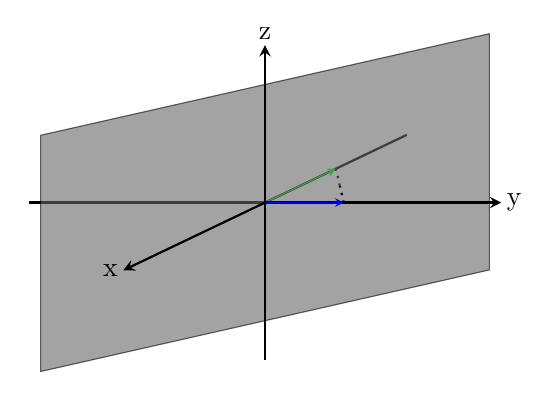
\begin{tikzpicture}[x={(-0.9cm,-0.43cm)}, y={(1cm,0cm)}, z={(0cm,1cm)}, scale=1.0,
    %Option for nice arrows
    >=stealth, %
    inner sep=0pt, outer sep=2pt,%
    axis/.style={thick,->},
    wave/.style={thick,color=#1,smooth},
    polaroid/.style={fill=black!60!white, opacity=0.6},
]
    % Colors
    \colorlet{darkgreen}{green!50!black}
    \colorlet{lightgreen}{green!80!black}
    \colorlet{darkred}{red!50!black}
    \colorlet{lightred}{red!80!black}

    % Frame
    \coordinate (O) at (0, 0, 0);
    \draw[thick] (-2,0,0) -- (O);
    \draw[thick] (0,-3,0) -- (O);
    \draw[green,->] (0,0,0) -- (-1,0,0);
    \draw[dotted,thick] (-0.5,0.5,0) -- (-1,0,0);

    \draw[polaroid]   (1.5, -1.5,  1.5) -- (-1.5, 1.5,   1.5)  -- (-1.5, 1.5, -1.5) -- (1.5, -1.5, -1.5) -- cycle;
    
    \draw[axis] (0,0,0) -- +(2, 0,   0) node [left] {x};
    \draw[axis] (0,0,0) -- +(0,  3, 0) node [right] {y};
    \draw[axis] (0,0,-2) -- +(0,  0,   4) node [above] {z};
    \draw[blue,->] (0,0,0) -- (0,1,0);
    \draw[dotted,thick] (0,1,0) -- (-0.5,0.5,0);

     %Crystal thin section


    %Second polarization


\end{tikzpicture}
\newpage
\section{Hypothetical Dataset}
\subsection{Life table}
In this practical, you will work with life tables. Read carefully the following text and do the exercise at the end of this section. The first part is the description of a hypothetical barn owl population and the second part is brief reminder of life table theory. 

\begin{figure}[h]
\centering
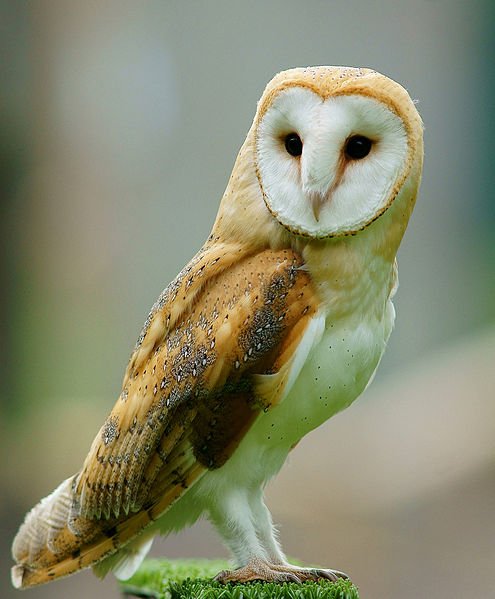
\includegraphics[width=0.3\textwidth]{Barnowl.jpg}
\caption{\label{fig:owl}Barn owl, from wikipedia.}
\end{figure}

\subsubsection{A barn owl population}
The barn owl (Schleiereule in German) is a common noctural prey bird (see fig. \ref{fig:owl}. In 2010, 10 female chicks were born and were followed over the years. In 2011, 8 of them were still alive. Only 3 females of this cohort reproduced in 2011: one produced 4 female chicks, one produces 3 female chicks and the last one produced 5 female chicks. In 2012 only 4 females were still alive. This time, they each produce 3 female chicks. In 2013, only one individual of the original cohort was still alive and had only one female chick. In 2014, all individuals were dead.   


\subsubsection{Standard cohort life table}

\begin{table}[h]
\centering
\begin{tabular}{ccccccc}
$x$ & $S(x)$ & $b(x)$ & $l(x)$ & $g(x)$ & Rep. rate \\\hline
$0$ &  $10$ & ... & ... & ...&...\\
$1$ & $8$ & ... & ... & ...&...\\
$2$ & ... & ... & ... & ...&...\\
$3$ & ... & ... & ... & ...&...\\
$4$ & ... & ... & ... & ...&...\\
\end{tabular}
\caption{\label{tab:LT}An example of a life table.}
\end{table}

Table \ref{tab:LT} contains the standard life-table calculation. Below is a description of each column. We purposefully do not provide you with the equations to obtain each value as this you will find yourself in the exercise. 
\begin{itemize}

\item \textit{The first column} $x$ is the age of the individuals. By convention, the newborn start at age $0$ and are age $1$ at their first birthday. 

\item \textit{The second column} $S(x)$ is the number of individuals of the cohort still alive at age $x$. 

\item \textit{The third column} $b(x)$ is the fecundity schedule (sometimes it is refered to as $m(x)$, \textit{m} for maternity). It is the \textbf{average number of female offspring born per unit of time to a female of a given age}. 

\item \textit{The fourth column} $l(x)$ is the survivorship schedule, not to be confused with the survival probability $g(x)$. It is defined as the \textbf{proportion of the original cohort that survives to a given age}. Or in other words it is the probability that an individual survives from birth to age $x$. 

\item \textit{The fifth column} $g(x)$ is the survival probability. It is different from the survivorship schedule in that it is the \textbf{probability that an individual of age $x$ survives to age $x+1$}. 

\item \textit{The sixth column} Rep. rate is what we call here the reproductive rate. We are in fact interested in the \textbf{net reproductive rate, $R_0$} but to find it, we must find the reproductive rate of each age. The net reproductive rate is defined as the \textbf{mean number of female offspring produced per female individual over their lifetime.} It is the reproductie potential of a female corrected for its mortality.
\end{itemize}

In addition to the elements of the table, there a few more important properties you can extract from the life table. A general property of the table is, $G$, the generation time. A definition of the generation time is \textbf{the average age of mothers when they give birth}. From the life table, you can also calculate the instantaneous rate of increase, $r$. Remember from Madan's lecture on unstructured population that:
\begin{equation}
N_t=N_0e^{rt}
\end{equation}
The exact solution of $r$ is given by solving the following equation adapted from the Lotka-Euler equation for $r$:
\begin{equation}
1=\sum\limits_{x=0}^k e^{-rx}l(x)b(x)
\end{equation}
This equation can only be solved iteratively. Alternatively, an approximation of $r$ is given by:
\begin{equation}
r \approx \frac{\ln(R_0)}{G}
\end{equation}


\begin{Exercise}[title=Life Table, label=LT, difficulty=1]
Write on paper a life table for the hypothetical barn howl population described above. Your life table should be organised like table \ref{tab:LT} and contain the same columns. For each column, write the corresponding equation. 

In addition, find $R_0$, $G$ and the approximation of $r$.
\end{Exercise}
\begin{Answer}[ref=LT]
The column $x$ and $S(x)$ are directly given in the text. 
\begin{equation}
b(x)=\frac{n(x)}{S(x)}
\end{equation}
where $n(x)$ is the number of female offspring produced by all the females of age $x$. $n(x)=\sum\limits_{i=1}^k{n(i)}$, where $n(i)$ is the number of female offrpsing per female of age $x$ in the cohort and $k$ the number of female age $x$ in the cohort.

\begin{equation}
l(x)=frac{S(x)}{S(0)}
\end{equation}

\begin{equation}
g(x)=frac{S(x+1)}{S(x)}
\end{equation}

\begin{equation}
Rep. rate=l(x)b(x)
\end{equation}
\begin{equation}
R_0=\sum\limits_{x=0}^k{l(x)b(x)}
\end{equation}
where $k$ is the maximum age. 

\begin{equation}
G=\frac{\sum\limits_{x=0}^k{l(x)b(x)x}}{\sum\limits_{x=0}^k{l(x)b(x)}}
\end{equation}
It may therefore be interesting to add an additional column to the table:
\begin{equation}
l(x)b(x)x=l(x)b(x)x
\end{equation}

% latex table generated in R 3.0.2 by xtable 1.7-3 package
% Mon Apr 14 14:59:14 2014
{\footnotesize
\begin{tabular}{rrrrrrr}
  \toprule 
 $x$ & $S(x)$ & $b(x)$ & $l(x)$ & $g(x)$ & Rep. rate & $l(x)b(x)x$ \\
 \midrule 
 0.00 & 10.00 & 0.00 & 1.00 & 0.80 & 0.00 & 0.00 \\ 
  1.00 & 8.00 & 2.00 & 0.80 & 0.50 & 1.60 & 1.60 \\ 
  2.00 & 4.00 & 3.00 & 0.40 & 0.25 & 1.20 & 2.40 \\ 
  3.00 & 1.00 & 1.00 & 0.10 & 0.00 & 0.10 & 0.30 \\ 
  4.00 & 0.00 & 0.00 & 0.00 &  & 0.00 & 0.00 \\ 
   \bottomrule 
\end{tabular}
}



\noindent$R_0=$ 2.9 \\$G=$ 1.483 \\$r=$ 0.7181 \\


\end{Answer}


\subsection{Age-structured Matrix Analysis}
In the former section, we have followed the fate of a hypothetical cohort of barn owls. Let us now look at the matrix. We want to know the number of individuals in each age class, thus we now shift from age to age class. Imagine these $10$ female barn owls are the founders of a new population and we do a postbreeding census, in which females are counted each year just after they have bred. Therefore, in year $2010$, there are $10$ of females in age class $1$. In $2011$ there are $8$ in  females in age class $2$ and $16$ females in age class $1$.  In $2012$ there are $4$ females in age class $3$, $13 females$ in age class $2$ and $12$ females produced by the individuals in age class $2$ and $26$ females produced by the females in age class $1$. In $2013$ there is $0$ female in age class $4$, there are $7$ females in age class $3$ and $30$ females in age class $2$. There are in addition $81$ new individuals in age class $1$; $1$ from the females in age class $3$, $19$ from the females in age class $2$ and $61$ from the females in age class $1$.

\begin{Exercise}[title=Age-structured matix, label=ASM, difficulty=1]
\Question Let us work out the matrix of this barn owl population on paper.
\subQuestion First, draw the life cycle of the population of barn owls describe above.
\subQuestion Find the survival probability $P_i$ for each age class $i$, that is the propability of an individual in age class $i$ to age class $i+1$. 
\subQuestion Find the fertility $F_i$, the average number of offpsring produced by an individual of age class $i$.
\subQuestion Write the equations to get the number of individuals in each age class at time $t+1$. Your equations should be of the form $n_1(t+1)=F_1n_1(t)$.
\subQuestion What is the structure of the corresponding Leslie matrix? What is the dimention of your matrix?
\subQuestion Build the corresponding Leslie matrix of this population.
\end{Exercise}

\subsubsection{Matrices in R}
Now that you have find the matrix of this population, let us implement it in R. Set the initial population vector to the founder population (10 individuals in age class $1$). 




\begin{knitrout}
\definecolor{shadecolor}{rgb}{0.969, 0.969, 0.969}\color{fgcolor}\begin{kframe}
\begin{alltt}
\hlcom{# Build the Leslie Matrix for the barn owl population}

\hlstd{F1}\hlkwb{<-} \hlcom{#insert your value here}
\hlstd{F2}\hlkwb{<-} \hlcom{#insert your value here}
\hlstd{F3}\hlkwb{<-} \hlcom{#insert your value here}
\hlstd{F4}\hlkwb{<-} \hlcom{#insert your value here}

\hlstd{P1}\hlkwb{<-} \hlcom{#insert your value here}
\hlstd{P2}\hlkwb{<-} \hlcom{#insert your value here}
\hlstd{P3}\hlkwb{<-} \hlcom{#insert your value here}
\hlstd{P4}\hlkwb{<-} \hlcom{#insert your value here }

\hlstd{A}\hlkwb{<-}\hlkwd{matrix}\hlstd{(}\hlkwd{c}\hlstd{(F1,P1,}\hlnum{0}\hlstd{,}\hlnum{0}\hlstd{,F2,}\hlnum{0}\hlstd{,P2,}\hlnum{0}\hlstd{,F3,}\hlnum{0}\hlstd{,}\hlnum{0}\hlstd{,P3,F4,}\hlnum{0}\hlstd{,}\hlnum{0}\hlstd{,P4),} \hlkwc{nr}\hlstd{=}\hlnum{4}\hlstd{)}
\hlstd{A}
\hlcom{# The initial population vector}

\hlstd{n11}\hlkwb{<-} \hlcom{#insert your value here}
\hlstd{n12}\hlkwb{<-} \hlcom{#insert your value here}
\hlstd{n13}\hlkwb{<-} \hlcom{#insert your value here}
\hlstd{n14}\hlkwb{<-} \hlcom{#insert your value here}

\hlstd{n0}\hlkwb{<-}\hlkwd{c}\hlstd{(n11, n12, n13, n14)}
\end{alltt}
\end{kframe}
\end{knitrout}


The next step is to project the population in the future. We have seen in the lecture that
\begin{equation}
n(t+1)=n(t)A
\end{equation}
To do so, we write the two following functions in R. The sign \%*\% is for matrix multiplication in R.
\begin{knitrout}
\definecolor{shadecolor}{rgb}{0.969, 0.969, 0.969}\color{fgcolor}\begin{kframe}
\begin{alltt}
\hlstd{n1}\hlkwb{<-}\hlstd{n0}\hlopt\hlstd{A}
\hlstd{nt2}\hlkwb{<-}\hlstd{A}\hlopt\hlstd{n0}
\end{alltt}
\end{kframe}
\end{knitrout}


Try run both lines. One is incorrect, why?

Next let us use this matrix to project the population. To do so we use a \texttt{for} loop over a specified time span. We first need to build an empty matrix which will be filled during the loop. The $n$ matrix is a matrix that has the same number of rows that the matrix $A$ and has as many column as the time span we set. Thus each column corresponds to one year. By first setting the time span to 4, check if we get the same population as the one described in the text. Then try different values of time span.


  


\begin{knitrout}
\definecolor{shadecolor}{rgb}{0.969, 0.969, 0.969}\color{fgcolor}\begin{kframe}
\begin{alltt}
\hlstd{tspan} \hlkwb{<-} \hlcom{#insert value                         # time span }
\hlstd{rows} \hlkwb{<-} \hlkwd{dim}\hlstd{(A)[}\hlnum{1}\hlstd{]}

\hlcom{# Build some matrices for storing eventual output}
\hlstd{n} \hlkwb{<-} \hlkwd{matrix}\hlstd{(}\hlnum{0}\hlstd{,rows,tspan)}     \hlcom{# empty matrix }

\hlstd{n[,}\hlnum{1}\hlstd{]} \hlkwb{<-} \hlkwd{c}\hlstd{( , , , )}           \hlcom{# insert value for the initial }
                              \hlcom{# population in each age class}

\hlcom{# Project population forward and store output}
\hlkwa{for} \hlstd{(t} \hlkwa{in} \hlnum{1}\hlopt{:}\hlstd{(tspan}\hlopt{-}\hlnum{1}\hlstd{)) \{}
    \hlstd{n[,t}\hlopt{+}\hlnum{1}\hlstd{]} \hlkwb{<-}\hlstd{A}\hlopt \hlstd{n[,t]}      \hlcom{# %*% = matrix multiplication in R}

\hlstd{\}}
\hlstd{n}
\end{alltt}
\end{kframe}
\end{knitrout}


Let us look at what happens to the 




\begin{knitrout}
\definecolor{shadecolor}{rgb}{0.969, 0.969, 0.969}\color{fgcolor}
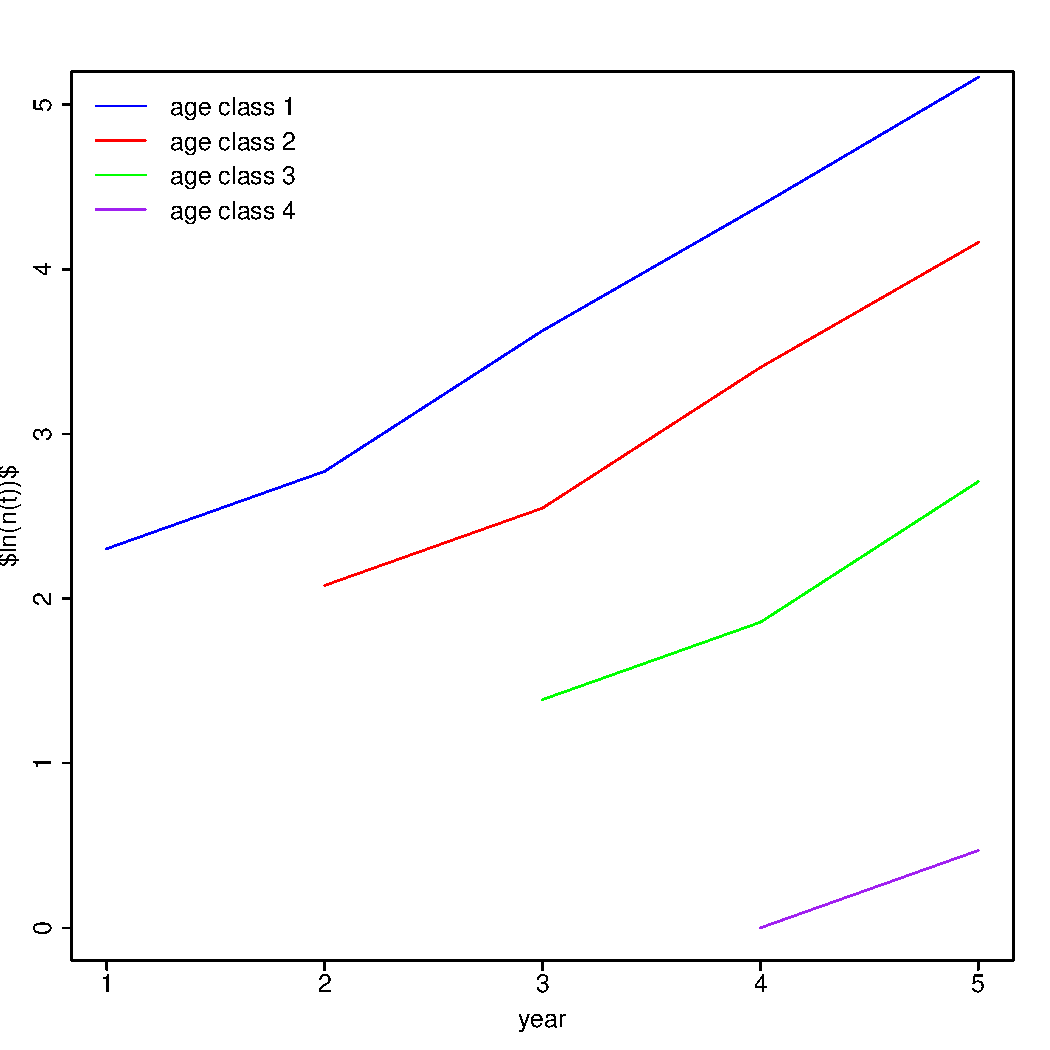
\includegraphics[width=\maxwidth]{figure/t3a} 

\end{knitrout}



\subsubsection{Asymptotic behaviour}

\subsubsection{Sensitivity analysis}

\subsubsection{Elasticity analysis}

\subsubsection{Transient dynamics}

\subsection{Stage-structured Matrix Analysis}

\subsection{Choice of bin size}
\section{Rotifer data}
Constructing matrices for the data from the lab practicals.
\shipoutAnswer
\end{document}
